\section{Hazard Function}

In the Calvo plus extension described in the problem set, the model essentially turns to the standard Calvo model. In that model, the firms only adjust with an exogenous probability (when the calvo fairy arrives). With $1-\alpha = 0.1$, we get that the probability of adjustment is always equal to 0.1. This can be seen in the Fig~\ref{hzcp}. The deviations towards the extremes of the x-axis are due to the fact that bins at those locations are relatively sparse.
\begin{figure}[H]
    \centering
    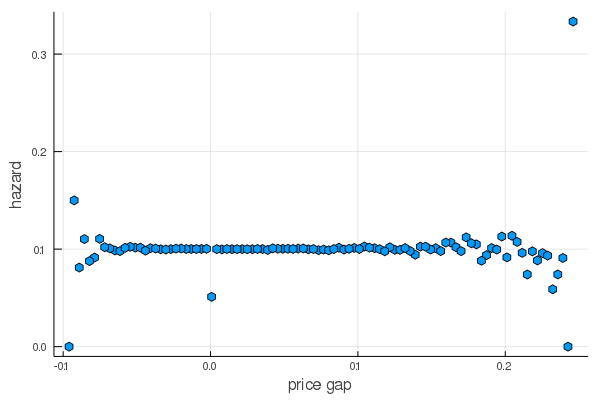
\includegraphics[width = 0.6\textwidth]{../tasks/Calvo_Plus/output/hazard_cp.png}
    \caption{Hazard}
    \label{hzcp}
\end{figure}

\section{Observed Price Change Distribution}

The observed price change distribution is shown in Fig~\ref{pccp}.
\begin{figure}[H]
    \centering
    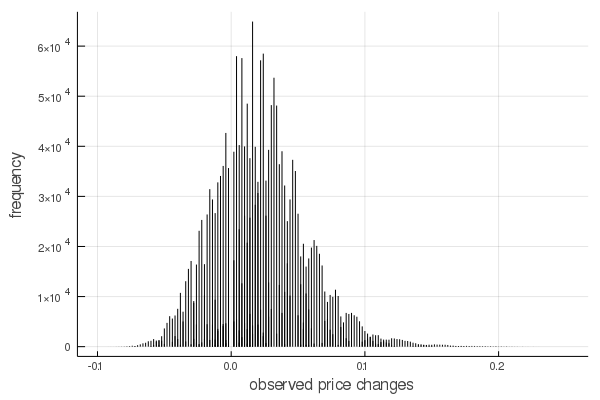
\includegraphics[width = 0.6\textwidth]{../tasks/Calvo_Plus/output/observed_p_changes_cp.png}
    \caption{Observed Price Changes}
    \label{pccp}
\end{figure}

\section{Price Gap Distribution }

The price gap distribution is shown in Fig~\ref{pgcp}.
\begin{figure}[H]
    \centering
    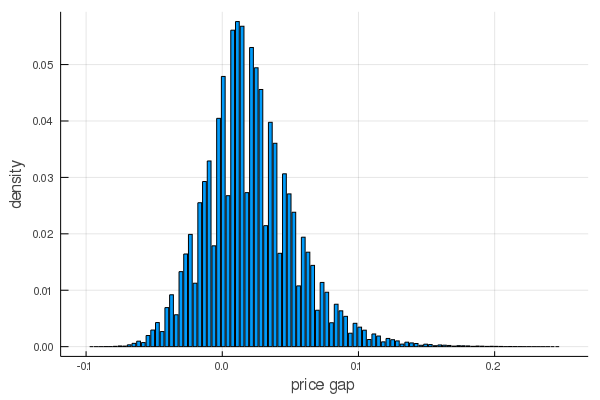
\includegraphics[width = 0.6\textwidth]{../tasks/Calvo_Plus/output/price_gap_dist_cp.png}
    \caption{Price Gap Distribution}
    \label{pgcp}
\end{figure}

\section{Impulse Response}

The IRF for the Calvo Plus economy is shown in Fig~\ref{irf11} and Fig~\ref{irf22}. Notice that this response is larger than in the Golosov-Lucas economy. Moreover, after the initial periods there is no variance in the relatively output and it fades away smoothly.


\begin{figure}[H]
    \centering
    \begin{minipage}{0.48\textwidth}
        \centering
        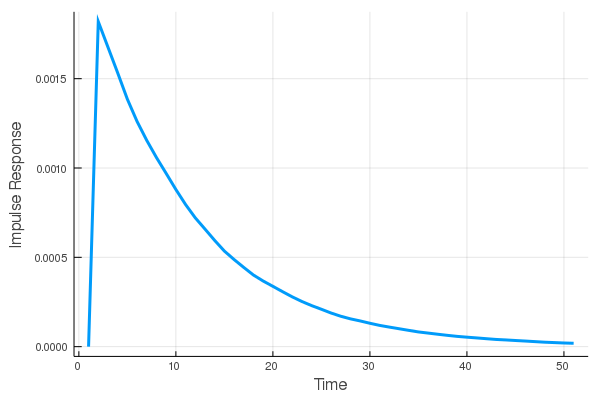
\includegraphics[width = \textwidth]{../tasks/Calvo_Plus/output/C_irf_50_periods.png}
        \caption{IRF till 50 periods after the shock}
        \label{irf11}
    \end{minipage}
    \begin{minipage}{0.48\textwidth}
        \centering
        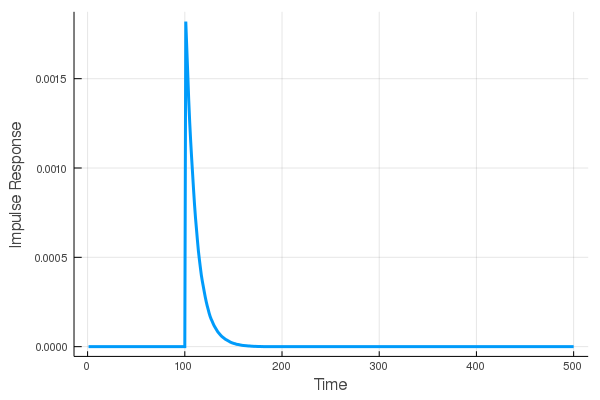
\includegraphics[width=\textwidth]{../tasks/Calvo_Plus/output/C_irf_500_periods.png}
        \caption{IRF for the entire simulation}
        \label{irf22}
    \end{minipage}
\end{figure}
